
%*****************************************
\chapter{Realisierung}\label{ch:Realisierung}
%*****************************************
    Bei der Realisierung einer AIDS müssen wie in~\autoref{ch:Grundlagen} beschrieben zwei Phasen durchlaufen werden.
    Die Trainingsphase und die Testphase.
    Diesen beiden Phasen liegt allerdings schon ein präparierter Datensatz und die Definition der exakten Eingaben und Ausgaben des \ac{LSTM} zu Grunde. 
    Welche Datensätze überhaupt in Frage kommen wurde bereits in~\autoref{sec:Datensatz} untersucht.
    Wie dieser weiterverarbeitet, für das \ac{LSTM} vorbereitet wird und welche Informationen neben dem Namen des System Calls verwendet werden könnte, 
    soll in~\autoref{sec:Preprocessing} betrachtet werden.
    Zuvor in~\autoref{sec:Tools} werden verschiedene Tools betrachtet, die für die Vorverarbeitung und weitere Implementierungen nötig sind.
    Der eigentliche Algorithmus, also das Finden von Anomalien in den Daten wird dann im~\autoref{sec:Algorithmus} beschrieben.
    Nachdem so also der verarbeitende Teil betrachtet wurde, soll in~\autoref{sec:StrukExp} die Strukturierung der Experimente präsentiert werden.
    Diese Strukturierung hat zum Ziel früh wenig vielversprechende Konfigurationen auszuschließen um ressourcenschonend Auswertungen durchzuführen.
    Speziell die Ressource Zeit, wie sich später zeigen wird, ist dabei im Rahmen dieser Arbeit eine Entscheidende.
    Abschließen soll dieses Kapitel dann in~\autoref{sec:Metriken} die Untersuchung von Metriken, welche dann für die Auswertung der Experimente benötigt wird.



    \section{Verwendete Tools}\label{sec:Tools}
        Tensorflow Keras
        Rechencluster clara
        sysdig

    \section{Vorverarbeitung}\label{sec:Preprocessing}
        %In dem kommenden Abschnitt~\ref{sec:struktur} wird die erste Vorverarbeitung des Datensatzes vorgestellt.
        Im kommenden Abschnitt~\ref{sec:syscalldarstellung} soll untersucht werden, welche Darstellungsformen für die eigentlichen System Calls interessant und sinnvoll sind.
        In dieser Arbeit werden die System Call Daten als Datenstream betrachtet.
        Weshalb in Abschnitt~\ref{sec:streamdarstellung} die Frage geprüft, wie dieser für das \ac{LSTM} dargestellt wird.
        Ein weiterer wichtiger Teil der Arbeit besteht darin, zu klären welche Metadaten neben dem Namen des System Calls noch verwendet werden können,
        um die Erkennungsrate zu erhöhen, bzw.\ die Fehlerrate zu verringern.
        Die Frage welche Informationen dafür verwendet werden können und wie diese dargestellt werden, soll in Abschnitt~\ref{sec:Meta}

        %\subsection{Vorverarbeitung des Datensatzes}\label{sec:struktur}
            %Gegeben 10 szenarien die aus bekannten CVEs bestehen.\
            %mit ca. 1000 files durschnittlich 45sec
            %in runs.csv genauere beschreibung files mit label und zeitangabe falls exploit
            %falls kein exploit dann exploit start time -1
            %keine dauer des exploits also ende nicht bekannt 
            %nicht systemcall genau start des angriffs angegeben 
            %führe puffer ein, da angegebener Zeitpunkt ungenau, sodass auch wirklich jeder angriff nach exploit start time
            %alles nach dem angrffszeitpunkt muss als anomalie gewertet werden, auch wenn angriff evtl noch nicht gestartet hat oder schon vorbei.
            %%TODO Quadranten
            %filtern von switch statements in Datensatz weil keine system calls
            %nur schließende syscalls keine öffnenden.
            %Muss wie in~\ref{sec:syscalls} beschrieben immer beide geben.
            %Schließende interessant, da auch Rückgabewerte betrachtet werden können

        \subsection{Wie wird ein System Call dargestellt?}\label{sec:syscalldarstellung}
            Neuronale Netze benötigen numerische werte deswegen Umwandlung von Namen der System Calls. 
            Eine einfache Kodierung dieser Strings bestünde darin die System Calls in Integer Werte umzuwandeln.
            Allerdings entstehen dabei künstliche Zusammenhänge und Ordnungen, welche für den Lernvorgang unvorteilhaft sein können~\cite{NEURALBISHOP1995}.
            Werden die System Calls als kategorische Daten betrachtet bietet sich das für neuronale Netze typische \ac{OHE} an.
            \paragraph{One-Hot-Encoding}
                Für die Darstellung eines System Calls mit dem \ac{OHE}, muss zunächst die Anzahl $n$ der unterschiedlichen System Calls ermittelt werden.
                Der System Call $sc_i$ aus der Menge der möglichen System Calls $ SC = \{sc_1,sc_2,\dots,sc_n\}$ 
                wird dann als Bit-Vektor $v_i$ der Länge $n$ kodiert.
                Dabei nehmen alle Stellen bis auf $i$ den Wert $0$ an und dort den Wert $1$.
                So wird aus dem System Call \textit{open} aus der Menge $SC = \{open, close, read\}$ der Vektor $v_1 = (1, 0, 0)$
                Da die Anzahl der möglichen System Calls und damit auch $n$ begrenzt ist, scheint diese Darstellung für einen System Call denkbar.
                Allerdings bringt sie auch zwei neue Probleme mit sich.
                Zum einen führt das \ac{OHE} eines System Calls bei großem $n$ zu einem langen und spärlich besetzten Vektor $v_i$.
                Gerade bei neuronalen Netzen führt das zu längeren Rechenzeiten.
                Und der neu gewonnen Vorteil, dass keine künstlichen Ordnungen vorhanden ist birgt den Nachteil, dass tatsächlich ebenso vorhandene Zusammenhänge verloren gehen.
                So besteht mindestens ein semantischer Zusammenhang zwischen \textit{open} und \textit{close} in der englischen Sprache, dieser ist in dem \ac{OHE} verloren gegangen. 
                Optimaler Weise gilt es also eine Darstellung zu finden die kurz ist und in der nur gewollte Ordnungen vorhanden sind.
                In der \ac{NLP} gilt es ähnliche Probleme durch die Darstellungen der Wörter zu lösen, zum Beispiel mit dem \ac{W2V} Verfahren.

            \paragraph{Word2Vec}
                Das \ac{W2V} Verfahren ist ein auf feedforward neuronalen Netzen basierender Ansatz, welcher häufig in der \ac{NLP} eingesetzt wird~\cite{W2VAYYADEVARA2018}.
                Dabei werden Wörter aus einem gegebenen Satz an möglichen Wörtern anhand eines Trainingsdatensatzes in dichte Vektoren $v$ fester Länge $embed\_size$ kodiert beziehungsweise \textit{embedded}\marginpar{zu dt.\ eingebettet}.
                Ziel des von~\cite{W2VMIKOLOV2013} eingeführten \ac{W2V} Verfahrens ist es eine Dimensionsreduktion durchzuführen, bei welcher möglichst viel Kontextinformationen erhalten bleiben.
                So sollen also die Vektordarstellungen von ähnlichen Wörtern ebenso ähnlich sein.
                Dies wird erreicht, indem Worte für das Erstellen der Kodierung nicht einzeln betrachtet werden, sondern immer in einem Kontext.
                Es wird angenommen, dass Wörter die häufig in einem ähnlichen Kontext auftreten, auch ähnlich sind.
                Wie umfangreich dieser Kontext für jedes Wort sein soll, wird mit der Fenstergröße $window\_length$ festgelegt.

                In der Trainingsphase gibt es zwei verschiedene Ansätze, zum einen das \textit{Continuous Bag-Of-Words},
                dabei wird versucht eine Vorhersage über ein Wort anhand des Kontextes zu machen.
                Hingegen wird unter Verwendung von \textit{Skip-gram}, eine Vorhersage des Kontextes aufgrund des Wortes vorgenommen.~\cite{EMBEDDINGPILEHVAR2020}

                Schwierigkeiten wie das häufige auftreten von Wörtern in der englischen Sprache wie \textit{the}, treten in der System Call Domäne nicht auf.
                Die Vorteile der dichtbesetzten und dimensionsreduzierten Vektoren machen sich auch bereits~\cite{IDSTHREADGRIMMER2021} in der anomaliebasierten \ac{HIDS} mit System Calls zu nutzen.
                Dieses Embedding wird auch im Folgenden verwendet.
                
            Neben den eigentlichen Namen der System Call enthalten tatsächliche System Calls wie in \autoref{sec:syscalls} beschrieben noch wesentlich mehr Informationen.
            Wie zumindest Teile dieser die Embeddings der System Calls erweitern können soll im folgenden Abschnitt untersucht werden.

            \subsection{Wie können weitere System Call Informationen dargestellt werden?}\label{sec:Meta}

                Wie zusätzliche Informationen der System Calls genutzt werden können ist auch Gegenstand bestehender Forschung.
                In \autoref{sec:related_sys_arg} wurden die verschiedenen bestehenden Ansätze untersucht.
                Im Folgenden soll es speziell darum gehen neue Darstellungsformen der System Call Argumente zu finden.
                Dabei soll noch einmal kurz auf die in \autoref{sec:syscalls} besprochenen Grundlagen zurückgegriffen werden um einen ersten Anhaltspunkt für wichtige Informationsquellen zu finden.

                Um die Unterscheidung von Normalverhalten und einer Anomalie zu erleichtern, müssen Faktoren betrachtet werden, welche sensibel auf eine Veränderung des Normalverhaltens reagieren.
                Gleichzeitig sollen dabei aber nicht einzelne Angriffe genutzt werden um diese Faktoren zu ermitteln.
                Denn dabei besteht die Gefahr Signaturen einzelner Angriffe abbilden zu wollen, was wie in \autoref{sec:Datenanalyse} ungewollte Nachteile hätte.
                Ziel dieses Abschnitts ist es die Überlegungen und Umsetzungen von zwei Verfahren zur Darstellung von zusätzlichen System Call Informationen zu präsentieren.

            \paragraph{Zeitliche Abstände von System Calls}

                Wie bereits in \autoref{sec:related_sys_arg} beschrieben verwenden Lucket et al.~\cite{TIMINGLUCKETT2016} die Timing-Information von System Calls für das Aufspüren von Rootkits.
                In diesem Abschnitt soll diese Idee wieder aufgegriffen werden und detaillierter beschrieben werden.
                Zwischenschieben von system call sequenzen um angriff zu verbergen.
                Verändert Timing der Normalabfolge.
                Statistik aus dem Datensatz:

                Schwierigkeiten Timing von System Calls hängt auch von Betriebssystem selbst ab.
                So werden indirekt auch Schedulerinformationen mitgelernt, was die Komplexität erhöhen kann und damit die Erkennung schwerer.
                
                Idee:
                Berechne größten Abstand zwischen zwei aufeinanderfolgende System Calls in den Trainingsdaten.
                Normiere folgende System Call Abstände mit diesem Maximum.
                So befinden sich die meisten Eingaben im Bereich von $[0,1]$ aber auch größere Werte möglich.

            \paragraph{Return Werte}


                \begin{figure}
                    \begin{subfig}{.5\textwidth}
                        \centering
                        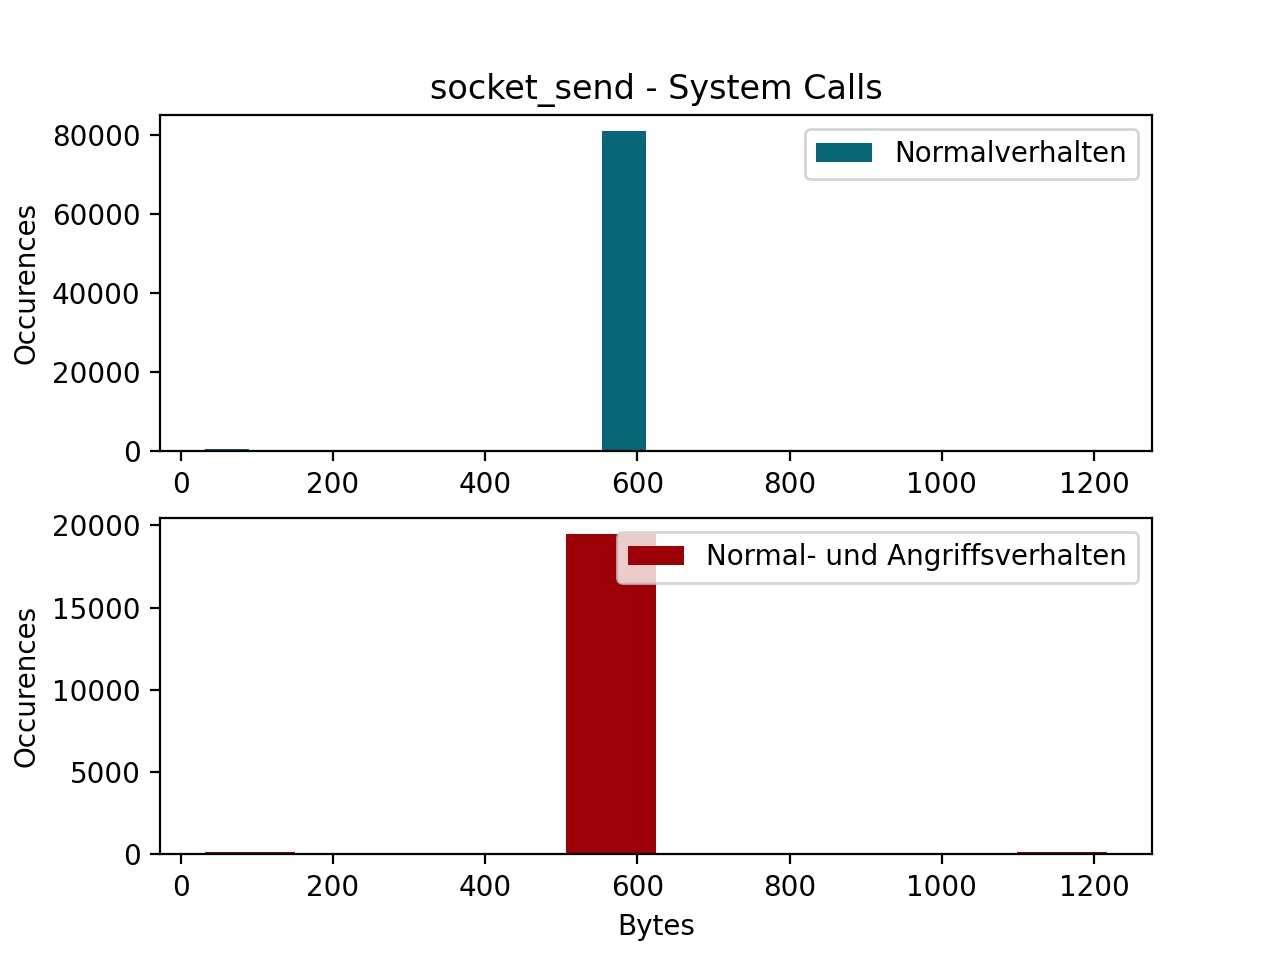
\includegraphics[width=0.5\textwidth]{images/fixCVE-2017-7529socket_send.jpg}
                        \caption{Einordnung des verwendeten \ac{IDS} (Relevant für diese Arbeit dicker markiert).}\label{fig:IDSOverview}
                    \end{subfig}
                    \begin{subfig}{.5\textwidth}
                        \centering
                        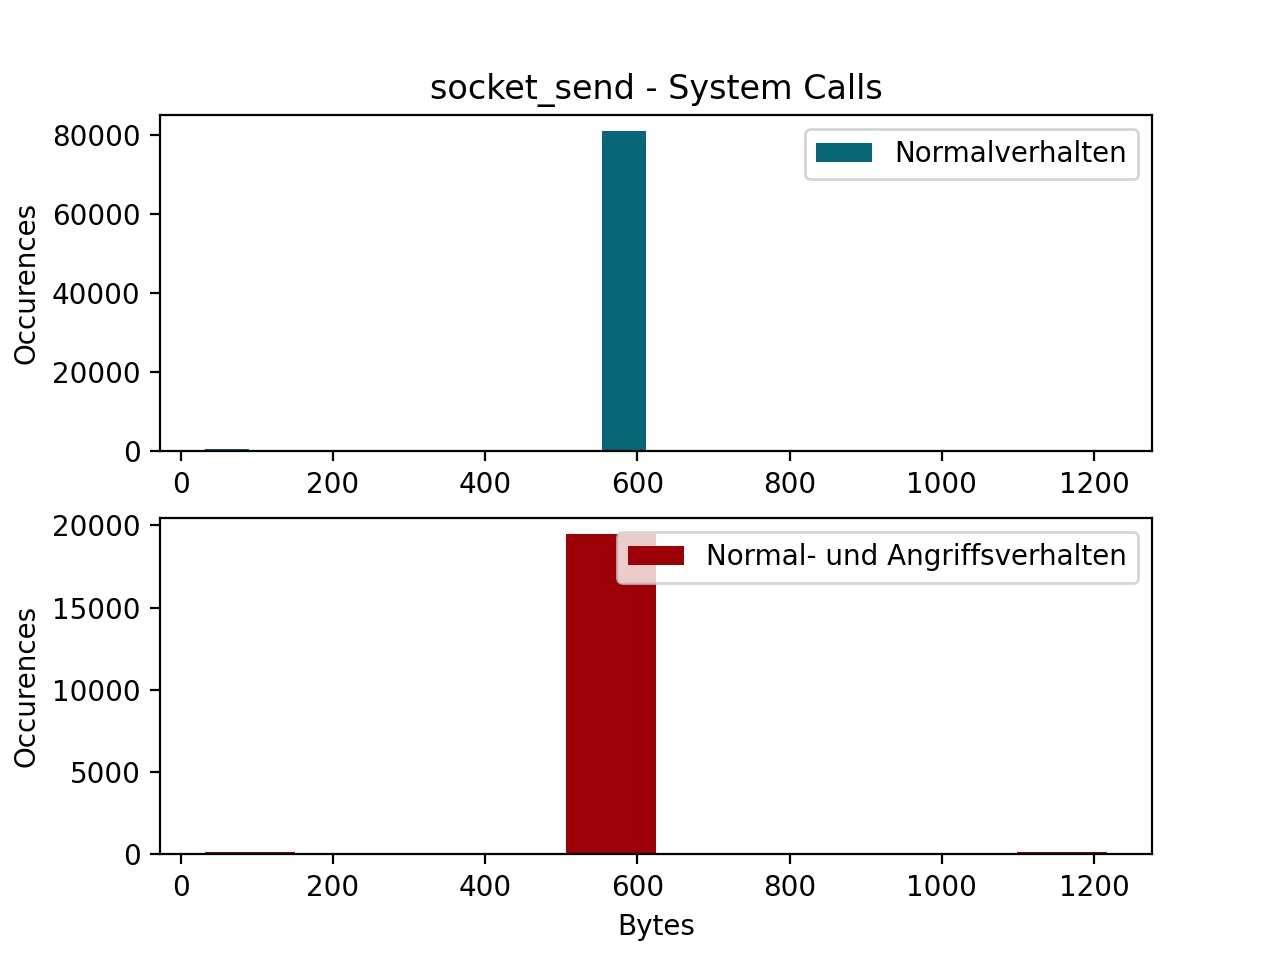
\includegraphics[width=0.5\textwidth]{images/fixCVE-2017-7529socket_send.jpg}
                        \caption{Einordnung des verwendeten \ac{IDS} (Relevant für diese Arbeit dicker markiert).}\label{fig:IDSOverview}
                    \end{subfig}
                \end{figure}
                Return Information
                    Anwendung kann viele Anfragen stellen, wie der Kernel darauf reagiert aber entscheident
                    Deswegen Reaktion in Form von return values embedden
                    gelesene und geschriebene bytes potentielle aussagekraft
%
        \subsection{Wie wird ein Datenstream dargestellt?}\label{sec:streamdarstellung}
            Erstellung von ngrammen bekannte Vorgehensweise.
            Aufteilen von Datenstream unbekannter Länge in feste Größe.
            Wird oft als \textit{Streaming Window} oder \textit{Ngram} bezeichnet.
            Nötig da \ac{LSTM} Eingaben fester Größe benötigen.
            %%%%NOTES
            % iterate syscalls 
            % Filter switch
            % Thread awareness ngrams
            % create embedding of syscall
            % append extra parameters

            \paragraph{Thread Awareness}
                Grimmer et al.~\cite{IDSTHREADGRIMMER2021} beschreiben in ihrer Arbeit wie die Thread Information der System Calls verwendet werden kann die Stream 
                Wie in \autoref{sec:syscalldarstellung} beschrieben enthalten  

                %und speziell von welchen System Calls diese Argumente kommen.spannend
                %Auch wenn ein allgemeiner Ansatz zur Kodierung wichtiger 
                %most frequent calls
                %Sql: vfrom, fcntl, lstat, nmap, poll
                %php: vfrom, fcntl, lstat, nmap, poll
                %bru: writev,read,  close, nmap, poll
                %eps: open,  read,  fstat, mmap, brk
                %zip: futex, write, getpid,protect,open
                %2019: statat,write, futex, stat, getpid
                %2014: writev,read,  nmap,  close,poll
                %2017: lwait,close,ollctl,write,writev
                %2018: statat,write, futex, getpid, stat


                %unique:
                    %vfrom, fcntl, lstat, nmap, poll, writev, read, close, open, fstat, mmap, brk
                    %futex, write, getpid, protect, statat, stat, lwait, ollctl

            %\begin{table}[ht]
                %\small
                %\label{tab:syscall}
                %\centering
                %\begin{tabular}{c||p{6cm}|p{3cm}|p{3cm}}
                    %\hline
                    %\rowcolor{Gray!36}
                    %\multicolumn{3}{c}{System Calls}\\
                    %\hline
                    %Name & Beschreibung & Interessante Argumente & return\\
                    %\hline
                    %\hline
                    %\rowcolor{Gray!16}
                    %fcntl & manipulate current fd & None & None
                    %\hline
                    %lstat & file status & path & 
                    %\rowcolor{Gray!16}
                    %mmap & map or unmap files or devices into memory & addr, length, fd,... & pointer to maped area
                    %poll & wait for event on fd & fds (fd, events, revents), timeout
                    %\rowcolor{Gray!16}
                    %open& Öffnet die in \textit{path} spezifizierte File und gibt einen \textit{file descriptor} zurück.& \textit{path}, \textit{flags}, \textit{mode} \\
                    %write& Schreibt bis zu \textit{count} Bytes aus dem Buffer (ab Stelle \textit{buf}) in die File, welche über den \textit{file descriptor}$fd$ definiert wird. & $fd$, $*buf$, \textit{count} \\
                    %\hline
                %\end{tabular}
                %\caption{Beschreibung ausgewählter System Calls}
            %\end{table}

                %Anzahl unique return Werte, nur numerische Werte betrachtet, 
                %res=-11(<f>/path/to/some/file) wird als -11 interpretiert
                %Bruteforce: 17192 2851 int, 14333 hex, 8 else
                %2012:       1897 193 int, 1698 hex, 6
                %2014:       16736 2706, 14022, 8
                %2017:       381 26, 354, 1 
                %2018:       110 106, 0, 4 
                %2019:       125 119 int werte und 6 else
                %SQL
                %EPS
                %PHP
                %Zipslip
%
                %Hinweis 3 Kategorien evtl kategorische Einteilung bei geringer Anzahl
                %Mögliche Bedeutungen bei else:
                    %Meist Fehlermeldungen!!!
                    %stat:
                        %file status, 
                        %sollte 0 bei success und -1 bei error, gefunden auch -2 
                    %ioctl:
                        %manipulate underlying device, 
                        %normalerweise 0 bei success manchmal negative werte
                        %-1 bei error
                        %manchmal return als ausgabe parameter
                    %Kategorische Betrachtung sinnvoll
                %HEX:\@
                    %mmap:
                        %map or unmap files into memory
                        %return pointer to mapped area
                    %brk:
                        %change data segment size
                        %return 0 on success -1 on error
                        %got hex value

                %Systemcalls welche Rückgabewerte haben:
                    %Bruteforce: {
                                 %'writev': 126627,
                                 %'read': 92587,
                                 %'munmap': 90757,
                                 %'close': 80535,
                                 %'poll': 64443,
                                 %'mmap': 45437,
                                 %'write': 39703,
                                 %'fcntl': 35722,
                                 %'brk': 30372,
                                 %'stat': 28356,
                                 %'semop': 27435,
                                 %'epoll_wait': 13746,
                                 %'fstat': 12950,
                                 %'shutdown': 11127,
                                 %'select': 11012, 
                                 %'lstat': 8060,
                                 %'getcwd': 4616,
                                 %'chdir': 4616,
                                 %'rename': 2308,
                                 %'connect': 4106,
                                 %'lseek': 1410                           ,
                                 %'clone': 1409,
                                 %'setgid': 705,
                                 %'setuid': 705}
                                 %'getdents': 40,

                    %2012: {
                            % 'read': 209140,
                            % 'futex': 149729,
                            % 'setsockopt': 148874,
                            % 'fcntl': 147382,
                            % 'write': 71308,
                            % 'pwrite': 25132,
                            % 'select': 7846,
                            % 'access': 3337,
                            % 'clone': 2523,
                            % 'mmap': 1723,
                            % 'poll': 1262,
                            % 'stat': 960,
                            % 'shutdown': 959,
                            % 'close': 959}
                            % 'munmap': 464,

                    %2014: {
                            % 'writev': 122406,
                            % 'munmap': 90471,
                            % 'read': 90368,
                            % 'close': 79167,
                            % 'poll': 62797,
                            % 'mmap': 44653,
                            % 'write': 38219,
                            % 'fcntl': 35692,
                            % 'brk': 28193,
                            % 'semop': 27166,
                            % 'stat': 26827,
                            % 'epoll_wait': 13629,
                            % 'fstat': 12290,
                            % 'shutdown': 11112,
                            % 'select': 11094,
                            % 'lstat': 7826,
                            % 'getcwd': 4324,
                            % 'chdir': 4324,
                            % 'connect': 4231,
                            % 'rename': 2162,
                            % 'clone': 1480,
                            % 'lseek': 1480,
                            % 'setgid': 740,
                            % 'setuid': 740,
                            % 'getdents': 34} 

                    %2017: {'epoll_wait': 53355,
                            % 'close': 52823,
                            % 'fstat': 26385,
                            % 'writev': 26110,
                            % 'sendfile': 26110,
                            % 'pread': 26109,
                            % 'write': 26109,
                            % 'recvfrom': 26108,
                            % 'getdents': 552,
                            % 'brk': 368,
                            % 'recvmsg': 330} 
                            % 'stat': 276,
                            % 'sendmsg': 166,
                            % 'futex': 92,

                    %2018: {
                            % 'write': 576100,
                            % 'futex': 262846,
                            % 'stat': 252081,
                            % 'read': 119433,
                            % 'close': 82304,
                            % 'fstat': 82226,
                            % 'select': 56420,
                            % 'setsockopt': 54836,
                            % 'ioctl': 54824,
                            % 'lseek': 54824,
                            % 'getsockopt': 27405,
                            % 'recvfrom': 27403,
                            % 'fcntl': 27396,
                            % 'poll': 4654,
                            % 'lstat': 3,
                            % 'pread': 3} 

                    %2019: {
                            % 'write': 542742,
                            % 'futex': 359158,
                            % 'stat': 307293,
                            % 'read': 136356,
                            % 'fstat': 81543,
                            % 'close': 81599,
                            % 'select': 75772,
                            % 'ioctl': 54282,
                            % 'setsockopt': 54269,
                            % 'lseek': 54250,
                            % 'fcntl': 27245,
                            % 'recvfrom': 27145,
                            % 'getsockopt': 27129,
                            % 'poll': 9050,
                            % 'lstat': 245,
                            % 'rename': 32,
                            % 'getdents': 32}
                            % 'unlink': 21,
                            % 'pread': 21,

                %ohe und w2v
                %word embedding parameterwahl wichtig $sqrt(distinct)$
                %Threadid kodieren: 
                %\begin{itemize}
                    %\item use entity embedding for ThreadID~\cite{GUO2016} 
                    %\item relationship between threads and reduce size (possible 1000 different threads)
                    %\item choose size of embedding -thumbrule $sqrt(unique value)$
                %\end{itemize}
                %zeit kodieren
                %\begin{itemize}
                    %\item use time delta of two different syscalls as new input
                %\end{itemize}
                %parameterlänge kodieren
                %\begin{itemize}
                    %\item syscall to int: Wandle Syscall name in Integer um
%
                     %ohe of sysint: use ohe for every syscall 
                     %n * (distinct calls + 1) eingabeneuronen 

                     %w2v von syscall
                     %weniger neuronen und nähe von syscall!!!
                    %\item ngram bilden: Bilde entsprechend angegebenes n ngramm
                %\end{itemize}
                %overhead berechnung embedding, muss allerdings nur einmal berechnet werden
                %zu erkennen w2v mit embedding size = 2  und window = 4 wesentlich schneller
                %embedding größer -> langsamer
                %vergleich ngram
                %im schnitt mit ngram gr 2 84\% von ngr 3 und 
                %w2v bringt entscheidenden Vorteil gegenüber ohe:
                %Jeweils vergleich der selben parameter außer w2v vs ohe:
                %Single small w2v nur 30\% der zeit gegenüber single small ohe
                %bei mulit w2v sogar nur 13\%
                %im mittel über alle architekturen 21.5\% der Zeit von ohe bei verwendung w2v

                %Anzahl unique return Werte, nur numerische Werte betrachtet, 
                %res=-11(<f>/path/to/some/file) wird als -11 interpretiert
                %Bruteforce: 17192 2851 int, 14333 hex, 8 else
                %2012:       1897 193 int, 1698 hex, 6
                %2014:       16736 2706, 14022, 8
                %2017:       381 26, 354, 1 
                %2018:       110 106, 0, 4 
                %2019:       125 119 int werte und 6 else
                %SQL
                %EPS
                %PHP
                %Zipslip
%
                %Hinweis 3 Kategorien evtl kategorische Einteilung bei geringer Anzahl
                %Mögliche Bedeutungen bei else:
                    %Meist Fehlermeldungen!!!
                    %stat:
                        %file status, 
                        %sollte 0 bei success und -1 bei error, gefunden auch -2 
                    %ioctl:
                        %manipulate underlying device, 
                        %normalerweise 0 bei success manchmal negative werte
                        %-1 bei error
                        %manchmal return als ausgabe parameter
                    %Kategorische Betrachtung sinnvoll
                %HEX:\@
                    %mmap:
                        %map or unmap files into memory
                        %return pointer to mapped area
                    %brk:
                        %change data segment size
                        %return 0 on success -1 on error
                        %got hex value

                %Systemcalls welche Rückgabewerte haben:
                    %Bruteforce: {
                                 %'writev': 126627,
                                 %'read': 92587,
                                 %'munmap': 90757,
                                 %'close': 80535,
                                 %'poll': 64443,
                                 %'mmap': 45437,
                                 %'write': 39703,
                                 %'fcntl': 35722,
                                 %'brk': 30372,
                                 %'stat': 28356,
                                 %'semop': 27435,
                                 %'epoll_wait': 13746,
                                 %'fstat': 12950,
                                 %'shutdown': 11127,
                                 %'select': 11012, 
                                 %'lstat': 8060,
                                 %'getcwd': 4616,
                                 %'chdir': 4616,
                                 %'rename': 2308,
                                 %'connect': 4106,
                                 %'lseek': 1410                           ,
                                 %'clone': 1409,
                                 %'setgid': 705,
                                 %'setuid': 705}
                                 %'getdents': 40,

                    %2012: {
                            % 'read': 209140,
                            % 'futex': 149729,
                            % 'setsockopt': 148874,
                            % 'fcntl': 147382,
                            % 'write': 71308,
                            % 'pwrite': 25132,
                            % 'select': 7846,
                            % 'access': 3337,
                            % 'clone': 2523,
                            % 'mmap': 1723,
                            % 'poll': 1262,
                            % 'stat': 960,
                            % 'shutdown': 959,
                            % 'close': 959}
                            % 'munmap': 464,

                    %2014: {
                            % 'writev': 122406,
                            % 'munmap': 90471,
                            % 'read': 90368,
                            % 'close': 79167,
                            % 'poll': 62797,
                            % 'mmap': 44653,
                            % 'write': 38219,
                            % 'fcntl': 35692,
                            % 'brk': 28193,
                            % 'semop': 27166,
                            % 'stat': 26827,
                            % 'epoll_wait': 13629,
                            % 'fstat': 12290,
                            % 'shutdown': 11112,
                            % 'select': 11094,
                            % 'lstat': 7826,
                            % 'getcwd': 4324,
                            % 'chdir': 4324,
                            % 'connect': 4231,
                            % 'rename': 2162,
                            % 'clone': 1480,
                            % 'lseek': 1480,
                            % 'setgid': 740,
                            % 'setuid': 740,
                            % 'getdents': 34} 

                    %2017: {'epoll_wait': 53355,
                            % 'close': 52823,
                            % 'fstat': 26385,
                            % 'writev': 26110,
                            % 'sendfile': 26110,
                            % 'pread': 26109,
                            % 'write': 26109,
                            % 'recvfrom': 26108,
                            % 'getdents': 552,
                            % 'brk': 368,
                            % 'recvmsg': 330} 
                            % 'stat': 276,
                            % 'sendmsg': 166,
                            % 'futex': 92,

                    %2018: {
                            % 'write': 576100,
                            % 'futex': 262846,
                            % 'stat': 252081,
                            % 'read': 119433,
                            % 'close': 82304,
                            % 'fstat': 82226,
                            % 'select': 56420,
                            % 'setsockopt': 54836,
                            % 'ioctl': 54824,
                            % 'lseek': 54824,
                            % 'getsockopt': 27405,
                            % 'recvfrom': 27403,
                            % 'fcntl': 27396,
                            % 'poll': 4654,
                            % 'lstat': 3,
                            % 'pread': 3} 

                    %2019: {
                            % 'write': 542742,
                            % 'futex': 359158,
                            % 'stat': 307293,
                            % 'read': 136356,
                            % 'fstat': 81543,
                            % 'close': 81599,
                            % 'select': 75772,
                            % 'ioctl': 54282,
                            % 'setsockopt': 54269,
                            % 'lseek': 54250,
                            % 'fcntl': 27245,
                            % 'recvfrom': 27145,
                            % 'getsockopt': 27129,
                            % 'poll': 9050,
                            % 'lstat': 245,
                            % 'rename': 32,
                            % 'getdents': 32}
                            % 'unlink': 21,
                            % 'pread': 21,

                %ohe und w2v
                %word embedding parameterwahl wichtig $sqrt(distinct)$
                %Threadid kodieren: 
                %\begin{itemize}
                    %\item use entity embedding for ThreadID~\cite{GUO2016} 
                    %\item relationship between threads and reduce size (possible 1000 different threads)
                    %\item choose size of embedding -thumbrule $sqrt(unique value)$
                %\end{itemize}
                %zeit kodieren
                %\begin{itemize}
                    %\item use time delta of two different syscalls as new input
                %\end{itemize}
                %parameterlänge kodieren
                %\begin{itemize}
                    %\item syscall to int: Wandle Syscall name in Integer um
%
                     %ohe of sysint: use ohe for every syscall 
                     %n * (distinct calls + 1) eingabeneuronen 

                     %w2v von syscall
                     %weniger neuronen und nähe von syscall!!!
                    %\item ngram bilden: Bilde entsprechend angegebenes n ngramm
                %\end{itemize}
                %overhead berechnung embedding, muss allerdings nur einmal berechnet werden
                %zu erkennen w2v mit embedding size = 2  und window = 4 wesentlich schneller
                %embedding größer -> langsamer
                %vergleich ngram
                %im schnitt mit ngram gr 2 84\% von ngr 3 und 
                %w2v bringt entscheidenden Vorteil gegenüber ohe:
                %Jeweils vergleich der selben parameter außer w2v vs ohe:
                %Single small w2v nur 30\% der zeit gegenüber single small ohe
                %bei mulit w2v sogar nur 13\%
                %im mittel über alle architekturen 21.5\% der Zeit von ohe bei verwendung w2v
                Thread information erweitern
                    Grimmer ngramme thread aware sinnvoll bei multithread anwendungen 
                    bei ihren verwendeted algorithmen ausreichend
                    für LSTM kontext wichtig, deshalb angeben ob aktueller thread aus selben Kontext wie der vorige kommt

                %Anzahl unique return Werte, nur numerische Werte betrachtet, 
                %res=-11(<f>/path/to/some/file) wird als -11 interpretiert
                %Bruteforce: 17192 2851 int, 14333 hex, 8 else
                %2012:       1897 193 int, 1698 hex, 6
                %2014:       16736 2706, 14022, 8
                %2017:       381 26, 354, 1 
                %2018:       110 106, 0, 4 
                %2019:       125 119 int werte und 6 else
                %SQL
                %EPS
                %PHP
                %Zipslip
%
                %Hinweis 3 Kategorien evtl kategorische Einteilung bei geringer Anzahl
                %Mögliche Bedeutungen bei else:
                    %Meist Fehlermeldungen!!!
                    %stat:
                        %file status, 
                        %sollte 0 bei success und -1 bei error, gefunden auch -2 
                    %ioctl:
                        %manipulate underlying device, 
                        %normalerweise 0 bei success manchmal negative werte
                        %-1 bei error
                        %manchmal return als ausgabe parameter
                    %Kategorische Betrachtung sinnvoll
                %HEX:\@
                    %mmap:
                        %map or unmap files into memory
                        %return pointer to mapped area
                    %brk:
                        %change data segment size
                        %return 0 on success -1 on error
                        %got hex value

                %Systemcalls welche Rückgabewerte haben:
                    %Bruteforce: {
                                 %'writev': 126627,
                                 %'read': 92587,
                                 %'munmap': 90757,
                                 %'close': 80535,
                                 %'poll': 64443,
                                 %'mmap': 45437,
                                 %'write': 39703,
                                 %'fcntl': 35722,
                                 %'brk': 30372,
                                 %'stat': 28356,
                                 %'semop': 27435,
                                 %'epoll_wait': 13746,
                                 %'fstat': 12950,
                                 %'shutdown': 11127,
                                 %'select': 11012, 
                                 %'lstat': 8060,
                                 %'getcwd': 4616,
                                 %'chdir': 4616,
                                 %'rename': 2308,
                                 %'connect': 4106,
                                 %'lseek': 1410                           ,
                                 %'clone': 1409,
                                 %'setgid': 705,
                                 %'setuid': 705}
                                 %'getdents': 40,

                    %2012: {
                            % 'read': 209140,
                            % 'futex': 149729,
                            % 'setsockopt': 148874,
                            % 'fcntl': 147382,
                            % 'write': 71308,
                            % 'pwrite': 25132,
                            % 'select': 7846,
                            % 'access': 3337,
                            % 'clone': 2523,
                            % 'mmap': 1723,
                            % 'poll': 1262,
                            % 'stat': 960,
                            % 'shutdown': 959,
                            % 'close': 959}
                            % 'munmap': 464,

                    %2014: {
                            % 'writev': 122406,
                            % 'munmap': 90471,
                            % 'read': 90368,
                            % 'close': 79167,
                            % 'poll': 62797,
                            % 'mmap': 44653,
                            % 'write': 38219,
                            % 'fcntl': 35692,
                            % 'brk': 28193,
                            % 'semop': 27166,
                            % 'stat': 26827,
                            % 'epoll_wait': 13629,
                            % 'fstat': 12290,
                            % 'shutdown': 11112,
                            % 'select': 11094,
                            % 'lstat': 7826,
                            % 'getcwd': 4324,
                            % 'chdir': 4324,
                            % 'connect': 4231,
                            % 'rename': 2162,
                            % 'clone': 1480,
                            % 'lseek': 1480,
                            % 'setgid': 740,
                            % 'setuid': 740,
                            % 'getdents': 34} 

                    %2017: {'epoll_wait': 53355,
                            % 'close': 52823,
                            % 'fstat': 26385,
                            % 'writev': 26110,
                            % 'sendfile': 26110,
                            % 'pread': 26109,
                            % 'write': 26109,
                            % 'recvfrom': 26108,
                            % 'getdents': 552,
                            % 'brk': 368,
                            % 'recvmsg': 330} 
                            % 'stat': 276,
                            % 'sendmsg': 166,
                            % 'futex': 92,

                    %2018: {
                            % 'write': 576100,
                            % 'futex': 262846,
                            % 'stat': 252081,
                            % 'read': 119433,
                            % 'close': 82304,
                            % 'fstat': 82226,
                            % 'select': 56420,
                            % 'setsockopt': 54836,
                            % 'ioctl': 54824,
                            % 'lseek': 54824,
                            % 'getsockopt': 27405,
                            % 'recvfrom': 27403,
                            % 'fcntl': 27396,
                            % 'poll': 4654,
                            % 'lstat': 3,
                            % 'pread': 3} 

                    %2019: {
                            % 'write': 542742,
                            % 'futex': 359158,
                            % 'stat': 307293,
                            % 'read': 136356,
                            % 'fstat': 81543,
                            % 'close': 81599,
                            % 'select': 75772,
                            % 'ioctl': 54282,
                            % 'setsockopt': 54269,
                            % 'lseek': 54250,
                            % 'fcntl': 27245,
                            % 'recvfrom': 27145,
                            % 'getsockopt': 27129,
                            % 'poll': 9050,
                            % 'lstat': 245,
                            % 'rename': 32,
                            % 'getdents': 32}
                            % 'unlink': 21,
                            % 'pread': 21,

                %ohe und w2v
                %word embedding parameterwahl wichtig $sqrt(distinct)$
                %Threadid kodieren: 
                %\begin{itemize}
                    %\item use entity embedding for ThreadID~\cite{GUO2016} 
                    %\item relationship between threads and reduce size (possible 1000 different threads)
                    %\item choose size of embedding -thumbrule $sqrt(unique value)$
                %\end{itemize}
                %zeit kodieren
                %\begin{itemize}
                    %\item use time delta of two different syscalls as new input
                %\end{itemize}
                %parameterlänge kodieren
                %\begin{itemize}
                    %\item syscall to int: Wandle Syscall name in Integer um
%
                     %ohe of sysint: use ohe for every syscall 
                     %n * (distinct calls + 1) eingabeneuronen 

                     %w2v von syscall
                     %weniger neuronen und nähe von syscall!!!
                    %\item ngram bilden: Bilde entsprechend angegebenes n ngramm
                %\end{itemize}
                %overhead berechnung embedding, muss allerdings nur einmal berechnet werden
                %zu erkennen w2v mit embedding size = 2  und window = 4 wesentlich schneller
                %embedding größer -> langsamer
                %vergleich ngram
                %im schnitt mit ngram gr 2 84\% von ngr 3 und 
                %w2v bringt entscheidenden Vorteil gegenüber ohe:
                %Jeweils vergleich der selben parameter außer w2v vs ohe:
                %Single small w2v nur 30\% der zeit gegenüber single small ohe
                %bei mulit w2v sogar nur 13\%
                %im mittel über alle architekturen 21.5\% der Zeit von ohe bei verwendung w2v

    \section{Algorithmus}\label{sec:Algorithmus}
        \ac{LSTM} Sprachmodell soll Wahrscheinlichkeit des nächsten System Calls vorhersagen, gegeben eines System Calls oder einer Sequenz von System Calls.
        Gab es in den Trainingsdaten die feste Menge $S = {1,\dots,N}$ an System Calls, so gibt $x=x_1\dots x_l \ (x_i\in S)$ die Sequenz an $l$ System Calls an.
        Jeder dieser System Calls bekommt im ersten Schritt einen Integerwert zwischen 1 und $N$.
        Taucht in den Testdaten nun ein noch nicht bekannter System Call $x_i$ auf, also $x_i \notin S$, so erhält dieser den vorläufigen Wert 0.
        Zu jedem Zeitpunkt wird $x_i$ der Input Layer übergeben.
        Dabei wird ein Embedding aus Abschnitt~\ref{sec:embedding} verwendet. 
        Mit den gegebenen Trainingsdaten kann nun das \ac{LSTM} mittels des \textit{back-propagation through time} (BPTT) trainiert werden.
        % Im ersten Schritt besteht dieses Embedding aus dem \textit{One hot encoding} (OHE).
        % In weiterer Ausführung werden dann zwei W2V Verfahren verwendet.
        % Wie in Kapitel \ref{Grundlagen:LSTM} bereits beschrieben wird, soll das LSTM mit den kodierten system calls aus dem Trainingsdatensatz trainiert werden.
        An der Ausgangs Layer befindet sich eine Softmax Aktivierungsfunktion.
        Diese wird verwendet um die Ausgabe zu normalisieren und damit die Wahrscheinlichkeitsverteilung des nächsten System Calls zu erhalten.
        Also $P\left(x_i|x_{1:i-1}\right)$ für alle $i$. 
        

        \subsection{Training}\label{sec:Training}
            Nächsten Syscall vorhersagen und überprüfen ob richtig vorhergesagt
        \subsection{Anomalieerkennung}\label{sec:Anomalieerkennung}
            Es kann also bei Auftreten des System Calls $x_i$ überprüft werden mit welcher Wahrscheinlichkeit $p$ dieser vorhergesagt wurde.
            Der eigentliche Anomalie-Score wird dann folgenderweise berechnet:
            \begin{equation}
                ascore = 1 - p
            \end{equation}
            Unterschreitet dieser einen Schwellwert so wird dies als eine Anomalie gewertet und ein Alarm angezeigt.
        \subsection{Schwellwertbestimmung}
            Um den zuvor erwähnten Schwellwert automatisch zu bestimmen, wird der Algorithmus auf die Validierungsdaten angewendet. 
            Dabei dient der höchste Wert dieser Daten dann als Schwellwert, da angenommen wird, dass mindestens alle Daten aus den Validierungsdaten harmlos sind und damit unter dem Schwellwert liegen sollten.
            Wichtig ist dabei dafür nicht die Trainingsdaten zu wählen, da eine starke Verzerrung der Schwellwertes durch Overfitting der Daten entstehen könnte. 
            Das würde bedeuten, dass nur sehr geringe Anomaliewerte auftreten und der Schwellwert sehr gering ist und damit die Gefahr für viele Fehlalarme besteht.

            Alternativ betrachte die x wahrscheinlichsten vorhergesagten system calls, falls tatsächlicher system call nicht dabei --> alarm
            x ermitteln, betrachte validierungsdaten und schaue ob schlechtestes x aussehen würde
            tatsächlich oft einmal schlechteste platzierung und automatische erkennung von x schwer.

            {\color{red} In Datensatzkapitel!}
            \paragraph{Problem des Datensatz}

                In den Testdaten sind \textit{malicious} \marginpar{zu dt.\ schädlich} Files beinhaltet, welche eine Information über den Angriffszeitpunkt liefert. 
                Jedoch gibt es bei einer malicious File im Gegensatz zu den normalen Files  vier mögliche Zuordnungen.
                %TODO Bild einfügen von Quadranten 
                Befindet sich der Anomaliescore unter dem Schwellwert kann von einem \textit{True Negative} eingestuft werden.
                Also es wurde korrekter weise kein Alarm vorhergesagt.
                Befindet sich der Anomaliescore vor dem Angriffszeitpunkt über dem Schwellwert liegt ein \textit{False Positive} vor.
                Es wurde ein Alarm gemeldet an einer Stelle an dem kein Angriff stattfand.
                Nach dem angegebenen Angriffszeitpunkt wird es allerdings schwieriger.
                Denn liegt der Anomaliescore nach dem Angriffszeitpunkt über dem Schwellwert, wird von einem \textit{True Positive}, also einem korrektem Alarm ausgegangen.
                Jedoch könnte da der Angriff schon vorbei sein, oder gar noch nicht gestartet sein.
                Es können nach dem Angriffszeitpunkt auch \textit{False Positive} oder \textit{False Negative} geben, welche allerdings nicht als solche erkannt werden können.
                Wie sich das auf die Auswertung der Ergebnisse auswirkt wird in Kapitel~\ref{sec:metrik} beleuchtet.

        \subsection{Parameterwahl}
            ngram länge
            lstm merkt sich vorherige syscalls aber hinzunahme von syscalls weitere info
            -> finden von sweet spot
            generell großes n viele alarme
            kleines n weniger alarme  vorteil \ac{LSTM}\@?
            wichtiger Parameter den es zu ermitteln gilt

    \section{Strukturierung der Experimente}\label{sec:StrukExp}
        Um aussagekräftige Experimente zu entwickeln müssen zuerst 
        überlegungen zur praktischen umsetzung gemacht werden
        dabei wird in ersten Tests klar, dass zeit hierbei eine große rolle spielen wird

        erste Tests also ausgelegt um Faktoren zu ermitteln, welche die auswertungen stark verlangsamen
        und diese ausschließen.

        \subsection{Faktor Zeit}

            zeit/dr als groesse und farbe von scatter plot
            batch size test und train x/y achse

            eingrenzen von moeglichen konfigurationen

            Berechnungszeiten aus verschiedenen Perspektiven relevant:
            soll live system werden
            begrenzte rechenleistung und viele Tests zur auswertung von parametern architektur etc
            erster test zur abschätzung diverser zeitl.\ faktoren:

            Faktoren:
            \begin{itemize}
                \item Architektur
                \item Verarbeitung Stream

                     ngram größe
                \item embedding
            \end{itemize}
        ngram größe, architektur und verwendung w2v statt ohe
        Grobe Abschätzung der Zeit, da Berechnungen auf Clustern ausgeführt werden von Auslastung beeinflusst werden.
        Klare Erkenntnisse:

            Single Small 50 neuronen eine schicht:
            Single Big 250 neuronen eine schicht
            multi 50 neuronrn 3 schichten

        erste Abschätzung von Nutzen von Thread 
        einführen von stateful sowie Batch Normalization

    \subsection{Optimale Parameter}

        \paragraph{Architektur}
            versch architekturen:
            Single Small 50 neuronen eine schicht
            Single Big 250 neuronen eine schicht
            multi small 20 neuronen 3 schichten
            multi big 50 neuronrn 3 schichten
            deep erste 50 sonst 20 6 schichten

            singlesmall 43\% von Deep
            insgesamt am schnellsten single small
            wie zu erwarten,  deep am langsamsten

            teste eine schicht viele neuronen 
            eine schicht wenige neuronen
            mehrere schichten mehrere neuronen / mit dropout dazwischen
            viele schichten wenige neuronen /mit dropout dazwischen

            auf Grund des zeitlichen Faktors fallen Deep und multibig weg
            Also zu testen:
            Single Small
            Single 
            Multi Small
            Multi 

        \paragraph{Hyperparameter}
            aktivierungs funktion
            -> dense layer with softmax or tanh
            batch size
            learning rate
            optimizer

        \paragraph{Ngram Größe}
            ngram größer -> langsamer

        \paragraph{Threadinfo}
            Hypothese:
            Threadinfos bringen was

            Einbinden von thread information auf verschiedenen wegen:
            Thread aware ngrams (tan)
            Thread aware ngrams for w2v (tanw2v)
            Thread change flag (tcf)

            varianten:
            tan
            tanw2v
            tcf
            tan tcf
            tan tanw2v
            tcf tanw2v
            tan tanw2v tcf

            ---> welcher dieser varianten am besten?

        \paragraph{Parameter}
            args
            time

            \ac{LSTM} ohne Threadinfos mit OHE
            LSTM mit W2V ohne Threadinfos (ngram)
            LSTM mit W2V mit Threadinfos (ngram)
            LSTM mit W2V threadaware mit Threadinfos (ngram)
            LSTM mit W2V threadaware mit Threadinfos (ngram) und threadchangeflag
            LSTM mit W2Vthreadaware mit Threadinfos (ngram) und threadchangeflag, spezialtraining
            --> LSTM final

            Manche angriffe verändern Sequenz von syscalls nicht
            Hypothese:
            verwende Parameter um erg zu verb

            LSTM final + strlen
            LSTM final + time delta
            LSTM final + strlen + time delta



\section{Metriken}\label{sec:Metriken}

    Auf Grund dessen Metrik False Alarm/ consecutive false alarm und Detection rate falls einmal pro malicious file in quadrant 4 -> HIT
    Wahl von Metriken in NN
    Precision, Recall, f-score, TNR, FNR, FPR

    problematisch:
    nicht auf systemcall genau gelabelt
    recall precision usw nur auf file ebene:
    alarm nach exploitstarttime wird immer als hit gewertet -> aber evtl angriff noch nicht begonnen
    oder angriff bereits vorbei
    ebenso umgekehrt, eig muss jeder nicht alarm nach exploitstart als FN gewertet werden
    weswegen filegenau geschaut wird
    vorteil des Datensatzes gegenüber anderen, immerhin exploitstart time

    ilarm in quadrant ---> image
